\documentclass[11pt, a4paper, onecolumn, oneside, final]{report}

\usepackage[margin=0.6in, bottom=0.7in]{geometry}
\usepackage{tocbibind}
\usepackage{natbib}
\usepackage{subfig}
\usepackage{float}
\usepackage{booktabs}
\usepackage{multirow}

\usepackage{hyperref}
  \hypersetup{
  	colorlinks=false,
  	pdfborder=0 0 0,
  	linkcolor=blue,
  	citecolor=black,
  	bookmarksopen=false,
  	bookmarksnumbered=true,
  	pdfstartview=FitH,
  	pdfview=FitH
	}
	
\usepackage{url}
  \urlstyle{same}

\usepackage{fancyhdr}

\usepackage{amsmath}
\usepackage{amsfonts}
\usepackage{bm}

\usepackage{listings}
\usepackage{xcolor}
\usepackage{pdfpages}
\usepackage[bahasa]{babel}
\usepackage[fixlanguage]{babelbib}

\definecolor{codegreen}{rgb}{0,0.6,0}
\definecolor{codegray}{rgb}{0.5,0.5,0.5}
\definecolor{codepurple}{rgb}{0.58,0,0.82}
\definecolor{backcolour}{rgb}{0.95,0.95,0.92}

\lstdefinestyle{mystyle}{
    backgroundcolor=\color{backcolour},   
    commentstyle=\color{codegreen},
    keywordstyle=\color{magenta},
    numberstyle=\tiny\color{codegray},
    stringstyle=\color{codepurple},
    basicstyle=\ttfamily\footnotesize,
    breakatwhitespace=false,         
    breaklines=true,                 
    captionpos=b,           
    keepspaces=true,                 
    showspaces=false,                
    showstringspaces=false,
    showtabs=false,                  
    tabsize=2,
    numbers=none
}

\lstset{style=mystyle}

\title{Tugas Kelompok 1\\Aljabar Numerik Kelas A\\Tahun Ajaran 2020/2021}
\author{Eko Julianto Salim, Hocky Yudhiono, Jonathan Nicholas}

\begin{document}
\begin{titlepage}
    \begin{center}\begin{figure}
            \begin{center}
                
\includegraphics[width=2.5cm]{makara.eps}
            \end{center}
        \end{figure}    
        \vspace*{0cm}
        \textbf{
        	UNIVERSITAS INDONESIA\\
        }
        
        \vspace*{1.0cm}
        % judul thesis harus dalam 14pt Times New Roman
        \textbf{Persamaan Non Linier dan Optimisasi} \\[1.0cm]

        \vspace*{2.5 cm}    
        % harus dalam 14pt Times New Roman
        \textbf{Laporan Tugas Kelompok 2} \\
        
        \vspace*{3 cm}
        \textbf{Kelompok A09} \\
        % penulis dan npm
        
\begin{table}[H]
        \centering
        \begin{tabular}{c c}
            Eko Julianto Salim & 1906350925\\
            Hocky Yudhiono & 1906285604 \\
            Jonathan Nicholas & 1906293133\\
        \end{tabular}
        \end{table}
        \vspace*{5.0cm}

        % informasi mengenai fakultas dan program studi
        \textbf{
        	FAKULTAS ILMU KOMPUTER\\
        	DEPOK \\
        	MEI 2021
        }
    \end{center}
\end{titlepage}

\section*{Pendahuluan}

Persamaan non-linier adalah persamaan rumit yang setiap \textit{terms}-nya bisa melibatkan lebih dari satu komponen variabel, ataupun bentuk-bentuk transendental yang memiliki bentuk kurva non-linier. Tentunya tidak setiap persamaan matematika sudah ditemukan metode analitik atau matematisnya. Karena adanya kemampuan komputasi menggunakan mesin, berbagai masalah tersebut sebagian besar diselesaikan dengan pendekatan numerik.

Tidak menutup kemungkinan juga adanya permasalahan-permasalahan lebih rumit yang timbul, seperti sistem persamaan non linier, optimisasi fungsi, serta batasan-batasan yang dapat diatur terhadap permasalahan optimisasi tersebut. Dalam laporan tugas kelompok ini, kami akan memberikan analisis dan eksplorasi yang kami temukan sembari menjawab pertanyaan-pertanyaan yang ada.

\section*{Isi}
Untuk referensi pertanyaan dari laporan ini mengikuti dokumen \texttt{TK2 Analisis Numerik} yang sudah diberikan. 

\subsection*{Bagian A}
\subsubsection*{A1.}

Asumsikan $r$ ialah akar dari persamaan fungsi $f$ yang diferensiabel atau $f(r) = 0$. Apabila berlaku $0 = f(r) = f'(r) = f''(r) = \cdots = f^{(m-1)}(r)$, tapi $f^{m}(r) \ne 0$. Kita sebut bahwa $f$ memiliki akar dengan multiplisitas $m$ di $r$.\\

\subsubsection*{Fungsi Pertama}

Perhatikan bahwa persamaan $f_1(x) = x^2 - \cos(\pi x)$ merupakan fungsi genap, berlaku $f_1(x) = f_1(-x) = (-x)^2 - \cos(-\pi x) = x^2 - \cos(\pi x)$, yang berarti bahwa fungsi ini simetris terhadap sumbu y. Diobservasi lebih lanjut, $f_1(0) = -\cos(0) = -1$, yang berarti $r \ne 0$. Sehingga fungsi $f_1(x)$ akan memiliki akar-akar sejumlah genap, serta berlaku bila suatu bilangan riil $r$ merupakan akar dari $f_1(x)$, maka $-r$ juga merupakan akarnya karena adanya sifat kesimetrisan ini.

Dari observasi sebelumnya, dapat disimpulkan bahwa hanya perlu dicari akar-akar pada interval $(0, \infty)$. Selanjutnya, karena fungsi $\cos(\pi x)$ memiliki \textit{range} pada interval $[-1, 1]$, maka nilai $x^2 - \cos(\pi x) > 0$, untuk $x > 1$, dan tidak mungkin akar-akar persamaan tersebut muncul untuk $x > 1$.

Selanjutnya, akan dicari nilai $f_1$ pada $x = 1$. Dapat ditulis $f_1(1) =  1 - \cos(\pi) = 1 - (-1) = 2$. Berdasarkan \textit{Intermediate Value Theorem}, benar bahwa akar-akar dari fungsi $f_1(x) = x^2 - \cos(\pi x)$ tersebut akan muncul setidaknya sekali pada interval $(0, 1)$.

Ambil turunan pertama fungsi $f_1$, yaitu $f_1'(x) = 2x + \pi \sin(\pi x)$. Tinjau interval $(0, 1)$, perhatikan bahwa \textit{range} fungsi $\sin(\pi x)$ berada pada interval $(0, 1)$. Pada koordinat polar, fungsi ini akan berada pada kuadran 1 dan 2 sehingga secara intuitif akan selalu bernilai positif. Lebih lanjut, maka $\pi \sin(\pi x) > 0$ dan $2x > 0$.

Berdasarkan sifat turunan pertama dari fungsi, karena selalu bernilai positif, maka $f_1$ ialah fungsi naik dalam interval $(0, 1)$. Berdasarkan semua observasi yang sudah dipaparkan, dapat disimpulkan bahwa $f_1$ hanya memiliki $1$ akar riil dalam interval $(0, 1)$ dan secara global memiliki $2$ akar riil yang keduanya berada pada interval $[-1, 1]$.

Untuk multiplisitas, kembali ke definisi pertama dan perhatikan turunan pertamanya. Sudah dibuktikan bahwa turunan pertamanya $f_1'(x) > 0, x \in (0, 1)$. Tentunya turunan dari fungsi genap adalah fungsi ganjil, maka turunan pertamanya $f_1'(x) < 0, x \in (-1, 0)$. Sehingga jelas bahwa $f_1'(r)$ dengan $r$ ialah akar dari persamaan ini tidak mungkin bernilai $0$. Sehingga multiplisitas untuk akar-akar ini ialah $1$. Lebih lanjut untuk verifikasi secara numerik, fungsi akan di-\textit{plot} dalam kalkulator grafik, didapatkan figur berikut.

\begin{figure}[h!]
    \centering
    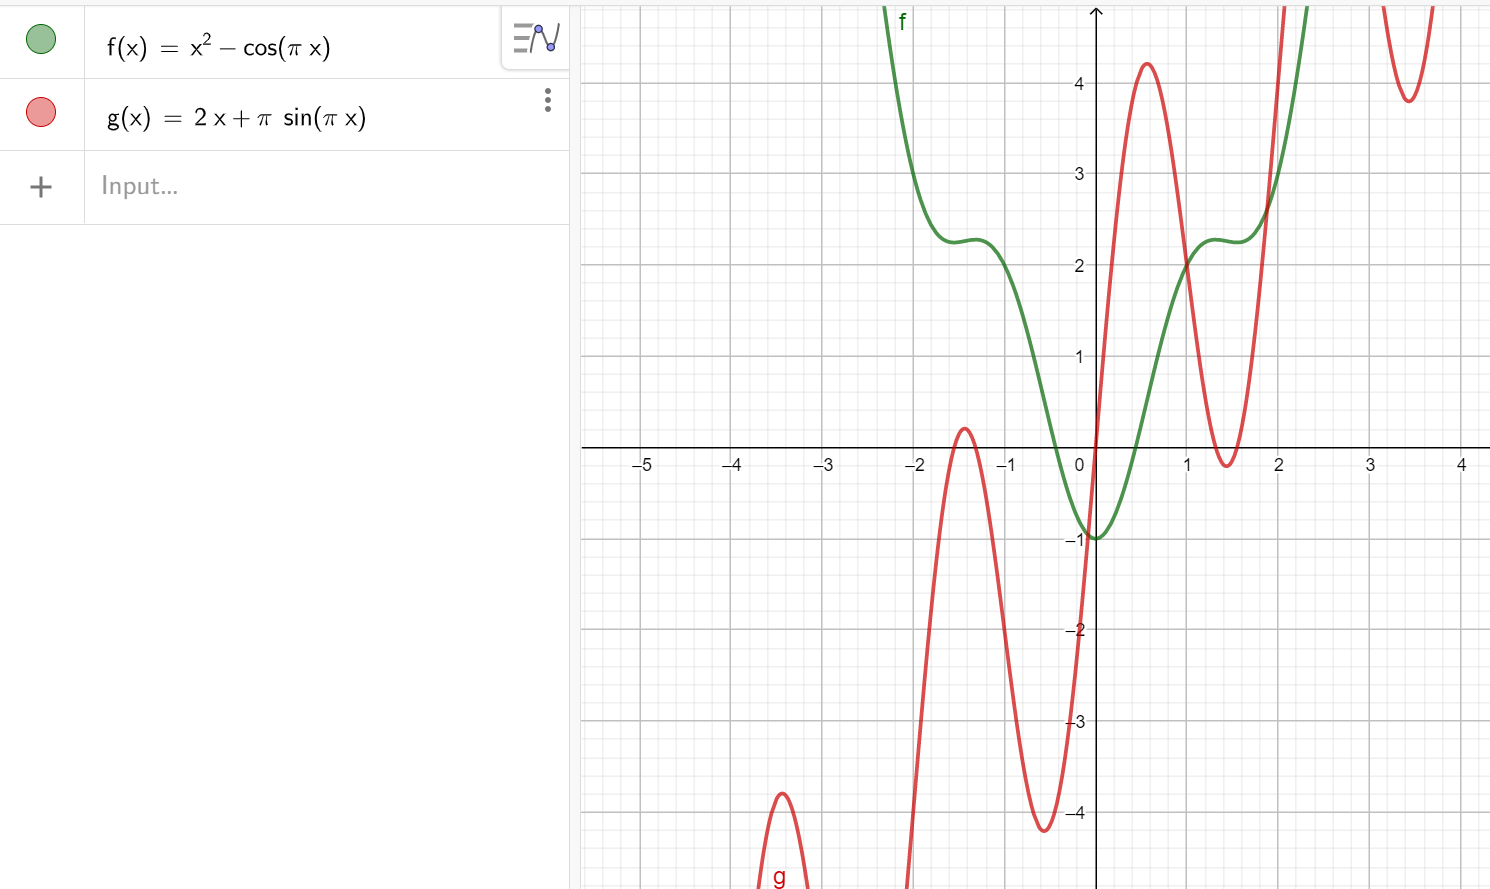
\includegraphics[width=0.3\textwidth]{assets/A1_1.png}
    \caption{Grafik Fungsi Pertama dan Turunannya}
\end{figure}

\subsubsection*{Fungsi Kedua}

Untuk persamaan $f_2(x) = x^x - x - 7 = \exp(x \ln x) - x - 7$ menggunakan pendekatan yang mirip dengan persamaan pertama. Pertama, definisikan domain untuk fungsi ini ialah $(0, \infty)$. Fungsi tersebut akan dibagi menjadi 2 interval, yaitu $(0, 1)$ dan $(1, \infty)$ karena mengetahui sifat fungsi eksponensial yang sensitif terhadap bilangan riil diantara $0$ dan $1$. Turunan pertama dari fungsi $f_2$ dapat dicari dengan langkah sebagai berikut.

$$
\begin{aligned}
    f_2 &= \exp(x \ln x) - x - 7\\
    df_2 &= d(x\ln x)\exp(x \ln x) - dx\\
    \frac{df_2}{dx} &= (1 + \ln x)\exp(x \ln x) - 1\\
    &= x^x(1 + \ln x) - 1
\end{aligned}
$$

Kita dapatkan nilai turunannya di $x = 1$, ialah $f_2'(1) = 1(1 + 0) - 1 = 0$. Selanjutnya untuk $x > 1$, diketahui fungsi akan bernilai positif. Berlaku $\ln x > 0$ dan $x^x > 1$, maka $f_2'(x) > 0$.

Hal ini berarti fungsi $f_2$ naik dalam interval $(1, \infty)$. Selanjutnya benar bahwa $f_2(1) = 1 - 1 - 7 = -7$, serta $\lim_{x \to \infty} f_2(x) = \infty$, sehingga berdasarkan \textit{Intermediate Value Theorem}, $f_2$ akan memiliki sebuah akar dalam interval $(1, \infty)$. Multiplisitasnya $1$, karena $f_2'$ nya positif untuk interval tersebut (tentunya $\ne 0$).

Untuk interval $(0,1)$, \textit{range} dari $x^x$ dan $x$ berada dalam interval $[0, 1]$, sehingga komponen $x^x - x$ akan berkisar antara [0, 1] juga. Lebih lanjut, $x^x - x \leq 1 \iff x^x - x - 7 \leq 1 - 7 = -6$ tidak mungkin memiliki akar riil pada interval (0,1). Jadi fungsi kedua ini hanya memiliki $1$ akar rill dan multiplisitasnya $1$. Lebih lanjut untuk verifikasi secara numerik, fungsi akan di-\textit{plot} dalam kalkulator grafik, didapatkan figur berikut.

\begin{figure}[h!]
    \centering
    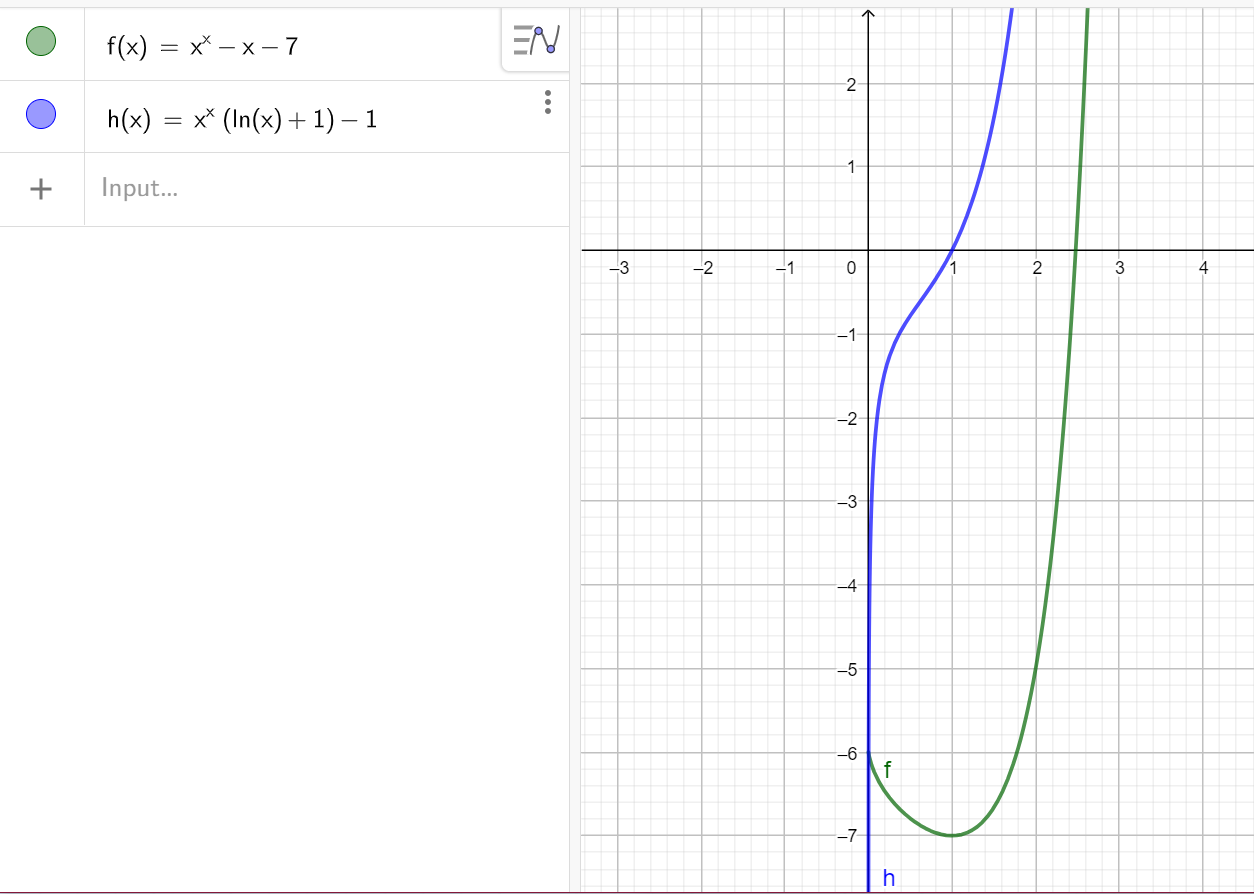
\includegraphics[width=0.3\textwidth]{assets/A1_2.png}
    \caption{Grafik Fungsi Kedua dan Turunannya}
\end{figure}

\subsubsection*{Fungsi Ketiga}

Untuk persamaan ketiga, dapat dilakukan pemfaktoran fungsi $f_3(x) = x^7+6x^6+2x^5-35x^4-19x^3+72x^2-27= (x-1)^2(x+3)^3(x^2-x-1)$. Cara melakukan pemfaktorannya ialah dengan menggunakan metode \textit{trial and error}, artinya memperhatikan konstanta yang umumnya merupakan kelipatan dari akar-akar dan menebak akar-akarnya, dilanjutkan dengan \textit{equation division} menggunakan \textit{long division} atau metode horner. Didapatkan sebanyak $4$ akar-akar persamaan, antara lain: $x = 1$ memiliki multiplisitas $2$, $x = -3$ memiliki multiplisitas $3$, serta dua akar irasional lainnya yang masing-masing memiliki multiplisitas $1$.

Untuk analisis lebih lanjut, bisa kita perhatikan turunan pertama dari fungsinya, yaitu $f_3' = 7x^6+36x^5+10x^4-140x^3-57x^2+144x = x(x - 1)(x + 3)^2(7x^2 + x - 16)$. Dari persamaan ini terlihat bahwa turunannya memiliki akar-akar dengan multiplisitas yang sesuai dengan yang sebelumnya. Turunan kedua fungsinya ialah $f_3'' = 42x^5+180x^4+40x^3-420x^2-114x+144 = 2 (x + 3) (21 x^4 + 27 x^3 - 61 x^2 - 27 x + 24)$ Dan turunan ketiganya $f_3''' = 210 x^4 + 720 x^3 + 120 x^2 - 840 x - 114$ yang tidak dapat difaktorkan kembali. Lebih lanjut untuk verifikasi secara numerik, fungsi akan di-\textit{plot} dalam kalkulator grafik, didapatkan figur berikut. Perlu diperhatikan bahwa perbandingan ukuran sumbu-x : sumbu-y ialah 1 : 50 untuk kemudahan visualisasi atas fungsi ini yang sangat sensitif terhadap nilai $x$.

\begin{figure}[h!]
    \centering
    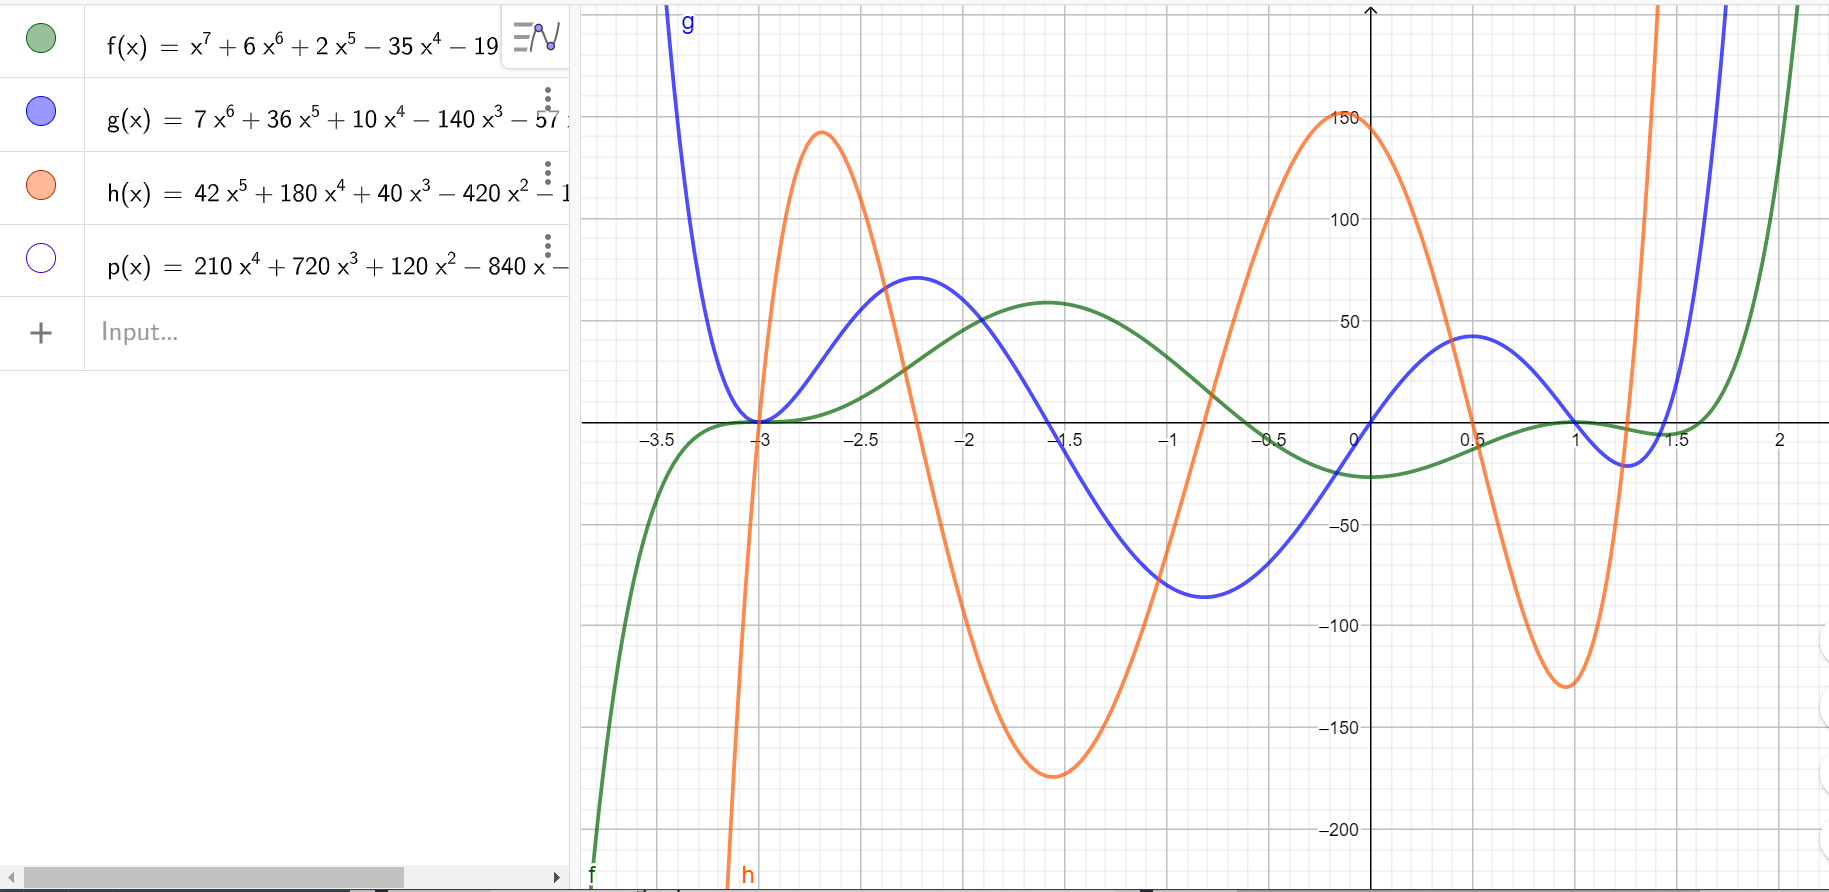
\includegraphics[width=0.5\textwidth]{assets/A1_3.png}
    \caption{Grafik Fungsi Ketiga dan Turunan-Turunannya}
\end{figure}

\subsubsection*{A2.}

Untuk ketiga persamaan tersebut akan dicari tahu akar-akar riilnya dengan tebakan yang bersesuaian. Perlu dicatat untuk metode \textit{bisection}, perlu adanya syarat bahwa interval yang diberikan memiliki tanda yang berbeda, yang berarti dapat dilakukan perbandingan dengan \textit{Intermediate Value Theorem}, sehingga kita dapat mencari tahu di titik mana fungsi tersebut bernilai 0.

Untuk metode newton sendiri, perlu dicari titik sehingga tidak ada iterasi yang menghasilkan nilai turunan $0$ (atau akan adanya pembagian dengan $0$), atau gradien horizontal. Setiap persamaan tersebut akan dicari menggunakan program yang dilampirkan, yaitu \texttt{A2\_1.m}, \texttt{A2\_2.m}, dan \texttt{A2\_3.m} berturut-turut untuk nomor persamaan yang bersesuaian.

Untuk persamaan pertama, didapatkan dua akar riil, yaitu sekitar $\pm 0.43843077948151$. Untuk persamaan kedua, didapatkan satu akar riil yaitu sekitar $2.478170814775$. Untuk persamaan terakhir, didapatkan empat akar-akar riil sekitar $-3, -0.61803398875, 1, 1.61803398875$. Secara berurutan untuk metode newton, akar-akar ini akan dipilih penebakan awalnya $-3.5, -0.5, 0.5, 2$.

Program yang mencari dengan \textit{subsection method} dibatasi kira-kira dengan potongan kode \texttt{(right-left < tolerance)}. Sementara newton dibatasi dengan \texttt{(abs(x - bf)*2 < tolerance)}.Potongan kode untuk newton ini memastikan bahwa selisih nilainya dan sebelumnya sudah cukup kecil perubahannya. Didapatkan tabel hasil iterasi sebagai berikut. Pada tabel tersebut baris ketiga ialah interval dan tebakan awal untuk masing-masing metode \textit{bisection} dan Newton.

\begin{table}[H]
\centering
\begin{tabular}{|c|c|c|c|c|c|c|}
\hline
\multirow{3}{*}{$k$} & \multicolumn{4}{c|}{Persamaan Pertama} & \multicolumn{2}{c|}{Persamaan Kedua} \\ \cline{2-7} 
& \multicolumn{2}{c|}{Bisection} & \multicolumn{2}{c|}{Newton's } & Bisection & Newton's \\ \cline{2-7} 
& (0.2, 0.8) & (-0.5, -0.1) & -0.6 & 0.4 & (1, 3) & 2 \\ \hline
2 & 6 & 6 & 2 & 2 & 8 & 5 \\ \hline
4 & 13 & 12 & 3 & 3 & 15 & 6 \\ \hline
8 & 26 & 26 & 4 & 4 & 28 & 7 \\ \hline
16 & 53 & 52 & 5 & 6 & 54 & 8 \\ \hline
\end{tabular}
\end{table}

\begin{table}[H]
\centering
\begin{tabular}{|c|c|c|c|c|c|l|c|c|}
\hline
\multirow{3}{*}{$k$} & \multicolumn{8}{c|}{Persamaan Ketiga} \\ \cline{2-9} 
 & \multicolumn{4}{c|}{Bisection} & \multicolumn{4}{c|}{Newton's} \\ \cline{2-9} 
 & (-4, -2.5) & (-1, -0.5) & (0.5, 1) & (1.5, 2) & -3.5 & -0.5 & 0.5 & 2 \\ \hline
2 & 8 & 6 & 6 & 6 & 11 & 3 & 7 & 5 \\ \hline
4 & 14 & 13 & 13 & 13 & 22 & 3 & 13 & 6 \\ \hline
8 & 28 & 26 & 26 & 26 & 45 & 4 & 27 & 7 \\ \hline
16 & 52 & 54 & 54 & 53 & 86 & 5 & 54 & 8 \\ \hline
\end{tabular}
\end{table}

Dari tabel tersebut, pada dasarnya metode bisection untuk setiap iterasinya akan memberikan sekitar 1 bit presisi lebih untuk nilainya. Tentunya untuk digit dalam desimal, atau basis 10, membutuhkan iterasi lebih. Secara analitis, dapat diaproksimasikan juga iterasi yang dibutuhkan, yaitu sekitar $\log_2(\frac{R - L}{TOL})$ untuk interval awal $[L, R]$, dan toleransi $TOL$.

Sementara untuk metode newton, presisi akan didapat cenderung lebih cepat. Hal ini karena metode newton ini secara matematis seringkali akan konvergen secara kuadrat dengan memanfaatkan \textit{fixed point iteration} dengan turunan. Namun ini juga tergantung dari persamaan yang didapat dan akar yang ingin dicari, karena bisa saja konvergensinya lebih lambat. Kapankah dia akan lebih lambat? Perhatikan tabel tersebut. Saat tebakannya bernilai $-3.5$, akan mendekati akar persamaan $-3$, hal ini berkaitan dengan multiplisitas dari persamaan, yang multiplisitasnya $3$ dan untuk tebakan $-0.5$ multiplisitasnya $2$.

Definisikan \textit{order of convergence} sebagai berikut. Bila \textit{error} yang didapatkan pada iterasi ke-$n$ ialah $|\epsilon_n| = k |\epsilon_{n+1}|^p$. Secara intuitif kita ketahui bahwa semakin banyak iterasi yang dilakukan maka \textit{error} yang akan didapatkan akan semakin kecil untuk fungsi yang errornya konvergen menuju $0$. Didapatkan \textit{order} atau ordo seberapa cepat \textit{error} tersebut mengecil, sebagai nilai $p$ dalam persamaan tersebut. Dalam metode \textit{bisection}, nilai $k = \frac{1}{2}$ dan $p = 1$.

Secara umum, metode newton memiliki nilai $p = 2$. Perhatikan pembuktian berikut. Dengan menuliskan suatu persamaan dalam ekspansi taylor-nya.

$$
f(\alpha )=f(x_{n})+f'(x_{n})(\alpha -x_{n})+{\frac {1}{2!}}f''(\xi _{n})(\alpha -x_{n})^{2}
$$

Karena $\alpha$ merupakan akar dari persamaan tersebut, maka berlaku:

$$
0=f(x_{n})+f'(x_{n})(\alpha -x_{n})+{\tfrac {1}{2}}f''(\xi _{n})(\alpha -x_{n})^{2}
$$

Selanjutnya bila komponen \textit{error} dipisahkan dan kedua ruas dibagi dengan $f'(x_n)$. Kemudian ingat kembali bahwa dalam metode newton, didefinisikan $x_{n+1} = x_n - \frac{f(x_n)}{f'(x_n)}$ maka akan didapatkan persamaan sebagai berikut.

$$
{\frac {f(x_{n})}{f'(x_{n})}+\left(\alpha -x_{n}\right)={\frac {-f''(\xi _{n})}{2f'(x_{n})}}\left(\alpha -x_{n}\right)^{2}
\iff
 \underbrace {\alpha -x_{n+1}} _{\varepsilon _{n+1}}={\frac {-f''(\xi _{n})}{2f'(x_{n})}}(\,\underbrace {\alpha -x_{n}} _{\varepsilon _{n}}\,)^{2}\,.}
$$

Dilanjutkan dengan persamaan galat.

$$
\left|{\varepsilon _{n+1}}\right|={\frac {\left|f''(\xi _{n})\right|}{2\left|f'(x_{n})\right|}}\cdot {\varepsilon _{n}}^{2}
$$

Saat nilai turunan di akarnya bernilai nol, jika dan hanya jika multiplisitas dari akar tersebut lebih dari satu, maka konvergensi dari \textit{error}-nya akan menjadi linear, dan tak lagi kuadratik. Hal ini menjelaskan mengapa untuk multiplisitas yang lebih tinggi metode ini lebih lambat dalam mendapatkan nilai akar-akar yang lebih presisi.

\subsubsection*{A3.}

Suatu titik $x_0$ disebut titik tetap dari suatu fungsi $f(x)$ jika dan hanya jika $f(x_0) = x_0$. Ide dari \textit{fixed point iteration} ini melakukan pendekatan solusi yang \textit{error}-nya konvergen menuju nol.

Persamaan yang tidak konvergen untuk persamaan pertama antara lain sebagai berikut.

$$
x = \frac{\cos(\pi x)}{x}; x = \sqrt{\cos(\pi x)}; x = \frac{(\cos^2(\frac{\pi x}{2}) - \sin^2(\frac{\pi x}{2}))}{x}; x = \frac{2 \cos^2(\frac{\pi x}{2}) - 1}{x}
$$

Persamaan yang konvergen antara lain sebagai berikut.

$$
x = \frac{\arccos(x^2)}{\pi}; x = \frac{2\arccos(\sqrt{\frac{x^2 + 1}{2}})}{\pi}
$$

\begin{figure}[h!]
    \centering
    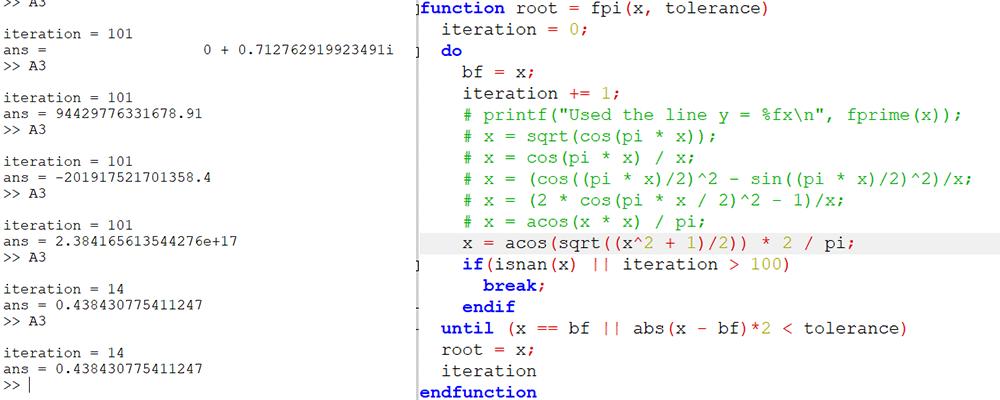
\includegraphics[width=0.4\textwidth]{assets/A3_1.png}
    \caption{Kode Demonstrasi}
\end{figure}

Menggunakan program \texttt{A3.m} dengan tebakan awal $0.43$, $0.8$ dan $0.2$ didapatkan bahwa benar bahwa persamaan-persamaan tersebut sesuai konvergenitasnya, untuk yang persamaan tidak konvergen, \textit{error}-nya ada yang semakin besar dan ada yang \textit{error}-nya tidak berubah, dan terjadi osilasi. Definisikan $r$ sebagai akar dari persamaan tersebut. Secara matematis, bisa dibuktikan juga bahwa bila persamaan \textit{fixed point iteration} $|g'(r)| < 1$ maka akan konvergen, dan benar saja secara matematis bahwa fungsi-fungsi yang tidak konvergen di atas memang memiliki nilai $|g'(r)| > 1$. Untuk membuatnya memiliki setidaknya memiliki \textit{convergence rate} dengan orde 2, maka haruslah $|g'(r)| = 0$.

Cara lainnya, kita bisa memanfaatkan metode steffensen yang tidak memerlukan turunan dan memanfaatkan properti \textit{fixed point} dan algoritma Aitken's $\Delta^2$ untuk mempercepat \textit{rate of convergence} suatu barisan. Berikut ialah rumusnya.

$$
AX = \frac{x_n x_{n+2} - x_{n+1}^2}{x_n + x_{n+2} - 2x_{n+1}}
$$

$$
(AX)_{n}=x_{n+2}-{\frac {(\Delta x_{n+1})^{2}}{\Delta ^{2}x_{n}}}=x_{n+2}-{\frac {(x_{n+2}-x_{n+1})^{2}}{(x_{n+2}-x_{n+1})-(x_{n+1}-x_{n})}}
$$

Algoritma steffensen melakukan komputasi dengan mencari nilai $x_{k + 1} = x_k - \frac{(g(x_k) - x_k)^2}{g(g(x_k)) - 2 g(x_k) + x_k}$ untuk setiap iterasinya. Metode ini memanfaatkan perkiraan konvergensi, sehingga akan menjadikan \textit{fixed-point iteration} yang awalnya linear kini menjadi kuadratik juga. Perhatikan kode \texttt{A3.m} didapatkan hasil galat dan iterasi sebagai berikut untuk tebakan awal $x_0 = 0.4$ yang akan mendekati akar $r \approx 0.43841$.

\begin{table}[H]
\centering
\begin{tabular}{|c|c|c|c|c|}
\hline
k       & 2 & 4 & 8 & 16 \\ \hline
Iterasi & 1 & 2 & 3 & 4 \\ \hline
\end{tabular}
\end{table}
 
\subsubsection*{A4.}

Untuk persamaan kedua, dapat dilakukan iterasi dengan \textit{secant method}. Dengan melakukan tebakan awal dua titik, dimanfaatkan \textit{secant line} yang merupakan garis yang memotong kurva persamaan di dua titik. Dari dua titik tersebut akan di-iterasi dan didapatkan titik ketiga, yang menjadi titik $x$ selanjutnya. Dapat dibuktikan bahwa \textit{rate of convergence}-nya tidak linear, namun juga tidak kuadratik. Dalam kasus ini, nilai $p$ sama dengan nilai \textit{golden ratio}.

$$
x_{n}=x_{n-1}-f(x_{n-1}){\frac {x_{n-1}-x_{n-2}}{f(x_{n-1})-f(x_{n-2})}}; p = \varphi ={\frac {1+{\sqrt {5}}}{2}}\approx 1.618
$$

Karena multiplisitas dari akar persamaan kedua ini satu, maka tebakan awal yang digunakan ialah $x_0 = 2; x_1 = 3$. Efisiensinya tidak terlalu berpengaruh karena interval tebakan kita yang cenderung kecil. \textit{Rate of convergence} justru tidak akan begitu terasa karena adanya nilai konstanta sendiri dari masing-masing tebakan awal untuk persamaan kedua. Dari beberapa iterasi, dengan toleransi masing-masing $k$ yang sama dengan eksperimen \texttt{A2}, didapatkan hasil sebagai berikut menggunakan program \texttt{A4.m}.

\begin{table}[H]
\centering
\begin{tabular}{|c|c|c|c|c|}
\hline
k       & 2 & 4 & 8 & 16 \\ \hline
Iterasi & 6 & 7 & 8 & 10 \\ \hline
\end{tabular}
\end{table}

Salah satu keuntungan dari metode ini ialah tidak diperlukannya turunan dari suatu fungsi dalam menghitung tebakannya. Apabila pencarian turunan sulit dilakukan ataupun mahal untuk dipanggil. Maka \textit{secant method} akan memberikan keuntungan flops secara signifikan.

\subsubsection*{A5.}

Untuk persamaan ketiga, akan dilakukan iterasi menggunakan metode newton yang sudah dimodifikasi dan didapatkan hasil sebagai berikut menggunakan program \texttt{A5.m}, yang secara berturut-turut mencari akar dengan nilai sekitar $-3, -0.61803398875, 1, 1.61803398875$, dan tebakan awal $x_0$ ada pada \textit{header} dari tabel tersebut. Akan digunakan persamaan sebagai berikut.

$$
x_{n + 1} = x_n - \frac{f(x_n) f'(x_n)}{f'(x_n)^2 - f(x_n) f''(x_n)}
$$

\begin{table}[H]
\centering
\begin{tabular}{|l|l|l|l|l|}
\hline
k & -3.5 & -0.5 & 0.5 & 1.5 \\ \hline
2 & 3 & 3 & 4 & 4 \\ \hline
4 & 4 & 4 & 4 & 6 \\ \hline
8 & 5 & 4 & 5 & 7 \\ \hline
16 & 6 & 5 & 6 & 8 \\ \hline
\end{tabular}
\end{table}

Menggunakan \textit{modified newton method} ini secara matematis akan lebih merugikan karena perlu dicari fungsi turunan kedua dari persamaan yang ingin dicari akar-akarnya. Namun, perhatikan bahwa untuk multiplisitas lebih dari satu, \textit{convergence rate}-nya akan jauh lebih baik, yaitu tetap kuadratik. Sehingga akan lebih menguntungkan bila kita sudah mengetahui sebelumnya jika akar yang kita cari memiliki multiplisitas lebih dari satu.

Pada dasarnya fungsi \textit{modified} ini memanfaatkan fakta bahwa turunan pertamanya bernilai $0$. Apabila kita misalkan $u(x) = \frac{f(x)}{f'(x)}$, kita gunakan properti yang menarik bahwa $f(x)$ akan mendekati $0$ lebih cepat dari $f'(x)$, oleh karena itu fungsinya akan tetap konvergen ke suatu titik, namun tentu saja akan lebih lambat karena $f'(x)$ \textbf{juga} akan menuju $0$. Inilah yang menyebabkan masalah karena multiplisitas $> 1$ berarti menyatakan $f'(x) = 0$. Kita bisa mendapatkan metode yang sudah dimodifikasi, yaitu $x_{n+1} = x_n - \frac{u(x_n)}{u'(x_n)}$. Dengan adanya fungsi ini, pada dasarnya \textit{rate of convergence}-nya akan bergerak lebih cepat. Apabila fungsi $u$ kita jabarkan, akan didapatkan persamaan awal yang digunakan dalam metode ini.

\subsubsection*{A6.}

Dalam membuat \textit{companion matrix} dapat menggunakan \textit{method} \texttt{compan(v)} pada \texttt{Octave}. \textit{Method} ini akan menerima sebuah vektor polinomial koefisien $\vec{v}$ dan mengembalikan \textit{companion matrix}-nya.

Akan dilakukan iterasi terhadap \textit{companion matrix} $A$ dengan rekurens $A_{k+1} = R_k Q_k$. Dengan $A_k = Q_k R_k$ yang merupakan dekomposisi QR dari matrix $A$. Perhatikan bahwa sebenarnya $A_{k+1} = R_k Q_k = Q_k^*A_kQ_k$. Disini trivial bahwa setiap rekurens tersebut menghasilkan matriks yang similar pada setiap iterasinya, yang artinya nilai eigen-nya sama. Dapat dibuktikan juga bahwa $\lim_{k \to \infty}A_k$ akan menjadi sebuah matriks segitiga atas, yang memiliki nilai eigen berupa diagonal-diagonal utamanya.

Meskipun pada awalnya matriks ini terlihat \textit{sparse}, apabila menggunakan \textit{Given's rotation} kompleksitasnya tidak $O(N^2)$ untuk setiap iterasi dalam melakukan dekomposisi QR-nya, karena lama kelamaan beberapa bagian yang awalnya nol pada \textit{companion matrix}-nya akan terisi juga. Sehingga akan dihitung sebagai $O(N^3K)$ dengan $K$ jumlah iterasi dalam metode QR tersebut. Namun dalam kasus ini, $N$ bernilai konstan sehingga iterasi sebanyak ratusribuan kali tidak akan menghabiskan banyak waktu. Dengan optimisasi tambahan, bisa digunakan Schur Decomposition yang langsung menghitung nilai $U'AU$.

Bila menggunakan QR \textit{iteration}, dalam 10 iterasi didapatkan sekitar ketepatan untuk 1 digit di belakang koma. Perhatikan program \texttt{A6.m}. Namun untuk mendapatkan ketepatan hingga 2 digit di belakang koma dibutuhkan sekitar $1000$ iterasi. Dalam $100000$ iterasi, didapatkan sekitar 6 digit di belakang koma. Konvergensinya sangat lambat, yaitu linear dengan konstanta sangat kecil. Lebih baik bila menggunakan \textit{Schur Decomposition} yang dalam $O(N^3)$ sudah mendapatkan ketepatan hingga 4 angka di belakang koma. Berikut ialah matriks setelah $10000$ iterasi. Terlihat bahwa entri-entri diagonal utamanya merupakan nilai-nilai eigen dari matriks \textit{companion} tersebut, yang sekaligus merupakan solusi dari fungsi polinomialnya.

$$
\begin{bmatrix}
-3.0006& -8.0021& -24.0480& 32.6726& -25.9602& 62.0672& 21.4120\\
 0.0000& -3.0000& -8.0154& 10.8886& -8.6570& 20.6804& 7.1320\\
 0& 0.0000& -2.9994& 3.6328& -2.8469& 6.9330& 2.4090\\
 0& 0& 0.0000& 1.6180& -0.8579& 1.8485& 0.6100\\
 0& 0& 0& 0.0000& 1.0001& -1.3473& -0.6489\\
 0& 0& 0& 0& 0.0000& 0.9999& -0.4404\\
 0& 0& 0& 0& 0& 0.0000& -0.6180\\
\end{bmatrix}
$$

\textit{Utility wise}, metode ini akan berguna bila persamaan yang ingin dicari banyak dan tidak perlu repot memerhatikan nilai tebakan awal dan konvergensi serta turunan dari suatu fungsi polinomial. \textit{Complexity wise}, apabila fungsi polinomial sederhana dan tidak banyak, maka lebih baik menggunakan metode \textit{newton-like root finding}, karena dari segi presisi lebih tepat dan tidak memerlukan banyak iterasi. Namun apabila kita perhatikan segi baiknya, kita bisa saja mengombinasikan keduanya, pertama-tama kita melakukan iterasi seadanya dengan menandai beberapa nilai eigen yang mungkin menjadi solusi dan menjadikannya sebagai tebakan awal untuk metode pencarian akar-akar seperti \textit{Newton's method}.

\subsection*{Bagian B}

Diberikan Sistem Persamaan Non-Linier berikut:

$$
\begin{aligned}
2u^2 - 4u +v^2 + 3vw^2 + 6w - 2 &= 0\\
u^2v + v^2 - 2v + 2w^2 - 3 &= 0\\
3u^2 - 12u + uv^2 + 3w^2 + 2 &= 0\\
\end{aligned}
$$

\subsubsection*{B1.}

Sebuah sistem persamaan non-linier umumnya akan sangat sulit diselesaikan dengan metode analitis. Salah satu cara yang bisa kita lakukan untuk memperoleh solusinya ialah dengan melakukan iterasi newton. 

Dalam pencariannya, rumus iterasi newton menjadi sebagai berikut.

$$
\vec{x}_{k+1} = \vec{x}_k - J_f(\vec{x}_k)^{-1} F(\vec{x}_k)
$$

Dengan $F(\vec{x}_k)$ ialah fungsi vektor dari sistem persamaan non linier, dan $J_f(\vec{x}_k)$ merupakan matriks Jacobian-nya. Dapat dibuat matriks yang sesuai dengan sistem persamaan non-linier tersebut sebagai berikut.

$$
F(u,v,w) = 
\left(
\begin{array}{ccc}
2u^2 - 4u + v^2 + 3vw^2 + 6w - 2\\
u^2v + v^2 - 2v + 2w^2 - 3\\
3u^2 - 12u + uv^2 + 3w^2 + 2\\
\end{array}
\right)
$$

$$
J_f(u,v,w) = 
\left(
\begin{array}{ccc}
 4 u-4 & 2 v+3 w^2 & 6 v w+6 \\
 2 u v & u^2+2 v-2 & 4 w \\
 6 u+v^2-12 & 2 u v & 6 w \\
\end{array}
\right)
$$

Bila diambil tebakan awal $\vec{x} = \begin{bmatrix}1 & 1 & 1 \end{bmatrix}^T$, maka akan didapatkan hasil akhir $\vec{x} = \begin{bmatrix}0.2397 & -0.9293 & 0.4070 \end{bmatrix}^T$ dalam sekitar 13 kali iterasi, kemudian \textit{error}-nya akan semakin mengecil, dan vektor galatnya akan konvergen menuju vektor nol. Berikut ialah persamaannya galatnya.

$$
y = F(0.2397, -0.9293, 0.4070) = 
\begin{bmatrix}
  -2.2204 \cdot 10^{-16}&
            0&
   4.4409 \cdot 10^{-16}
\end{bmatrix}^T
$$

\begin{table}[H]
\centering
\begin{tabular}{|c|c|c|c|c|c|}
\hline
\textbf{Iterasi} & \textbf{Galat} & \textbf{Iterasi} & \textbf{Galat} & \textbf{Iterasi} & \textbf{Galat} \\ \hline
$1$ & $125.9760$ & $6$ & $1.0536$ & $11$ & $2.2204 \cdot 10^{-16}$ \\ \hline
$2$ & $33.3093$ & $7$ & $0.1875$ & $12$ & $4.4409 \cdot 10^{-16}$ \\ \hline
$3$ & $8.8251$ & $8$ & $1.7485 \cdot 10^{-2}$ & $13$ & $4.9651 \cdot 10^{-16}$ \\ \hline
$4$ & $3.0136$ & $9$ & $9.5424 \cdot 10^{-5}$ &  & \\ \hline
$5$ & $1.3970$ & $10$ & $9.4813 \cdot 10^{-10}$ &  &  \\ \hline
\end{tabular}
\end{table}

Galatnya bernilai $||y||_2 \approx 4.9651 \cdot 10^{-16}$. Selain itu, sistem persamaan non linear tersebut tidak hanya memiliki satu solusi. Saat tebakan awal $\vec{x} = \begin{bmatrix}5 & 5 & 5 \end{bmatrix}^T$, maka akan didapatkan hasil akhir $\vec{x} = \begin{bmatrix}0.7995 & 2.1228 & -0.8314 \end{bmatrix}^T$ dalam sekitar 13 kali iterasi, ada pula hasil yang berbeda saat diambil tebakan awal $\vec{x} = \begin{bmatrix}-2 & -2 & -2 \end{bmatrix}^T$. Untuk tebakan awal sendiri bisa diambil vektor yang mana saja, asalkan hasil $F(\vec{x})$ konvergen menuju $0$ saat iterasinya semakin banyak.

\subsubsection*{B2.}

Pada metode newton, beberapa kekurangannya ialah jawabannya sensitif terhadap nilai awal, tidak seperti metode \textit{gradient descent}, selanjutnya metode ini sangatlah mahal sebenarnya. Dalam setiap iterasinya diperlukan sekitar $O(N^3)$ flops. Untuk menghitung beberapa matriks yang besar, tentunya ini akan sangat memakan \textit{resource}.

Akan digunakan metode BFGS yang merupakan turunan dari metode quasi-newton. Pada dasarnya metode ini digunakan ketika turunan atau matriks Hessian sangat sulit untuk ditemukan. Salah satu caranya ialah dengan menggunakan aproksimasi terhadap matriks Hessian yang diperbarui untuk setiap iterasi.  Misalkan matriks ini sebagai matriks $B$ yang merupakan matriks positif definit. Tentunya saat kita melakukan pembaharuan matriks $B$ ini, kita melakukannya dalam kompleksitas yang lebih kecil, yaitu $O(N^2)$. Implementasinya terdapat pada kode \texttt{B2.m}.

Untuk menentukan titik awalnya cukup sulit, karena sangat sensitif fungsinya. Maka setelah dilakukan pengacakan titik tebakan awal beberapa kali, ditemukan beberapa titik yang galatnya akan konvergen ke nol, yaitu $\vec{x}_0 = \begin{bmatrix} 0.5111 \\
  0.4755\\
  1.8644\end{bmatrix}$ yang akan konvergen ke $\vec{x}_0 = \begin{bmatrix} 0.2397 \\
  -0.9293\\
   0.4070\end{bmatrix}$.

Bila fungsi yang ingin dicari tidak bisa ditemukan turunannya, maka gunakan aproksimasi matriks awal $B$ matriks identitas $\textit{I}$. Namun, apabila fungsi yang ingin dicari bisa dihitung Hessian-nya, alangkah lebih baik bila kita menggunakan Hessian-nya di awal. Untuk perkembangan lebih lanjut, bisa saja untuk setiap kelipatan $c$ iterasi dihitung ulang Hessian-nya. Berikut ialah hasil 20 iterasi pertama untuk tebakan awal tersebut.

\begin{table}[H]
\centering
\begin{tabular}{|c|c|c|c|c|c|}
\hline
\textbf{Iterasi} & \textbf{Galat} & \textbf{Iterasi} & \textbf{Galat} & \textbf{Iterasi} & \textbf{Galat} \\ \hline
$1$ & $3.9403$ & $8$ & $0.4135$ & $15$ & $1.1120 \cdot 10^{-7}$ \\ \hline
$2$ & $2.0257$ & $9$ & $0.2426$ & $16$ & $5.1621 \cdot 10^{-10}$ \\ \hline
$3$ & $1.2290$ & $10$ & $0.029207$ & $17$ & $2.1442 \cdot 10^{-13}$ \\ \hline
$4$ & $1.1534$ & $11$ & $5.6492 \cdot 10^{-3}$ & $18$ & $4.4409 \cdot 10^{-16}$ \\ \hline
$5$ & $1.9057$ & $12$ & $3.1076 \cdot 10^{-4}$ & $19$ & $6.2804 \cdot 10^{-16}$ \\ \hline
$6$ & $1.0263$ & $13$ & $7.1396 \cdot 10^{-5}$ & $20$ & $0$ \\ \hline
$7$ & $6.6797$ & $14$ & $9.6379 \cdot 10^{-6}$ &  &  \\ \hline
\end{tabular}
\end{table}

\subsection*{Bagian C}

Fungsi 1
$$
f(x,y) = x^2 - xy + y^2 + e^{xy}
$$
$$
\nabla f(x,y) = \{y e^{x y}+2 x-y, x e^{x y}-x+2 y\}
$$
Fungsi 2
$$
g(w,x,y,z) = (w+1)(x+1) + (x+1)(y+1) + (y+1)(z+1) - w^2 - x^2 - y^2 - z^2
$$
$$
\nabla g(w,x,y,z) = \{-2w + x + 1, w-2 x+y+2, x-2 y+z+2, y-2 z+1\}
$$

\subsubsection*{C1.}
Akan dilakukan \textit{steepest gradient descent} untuk mencari titik optimum. Pada dasarnya \textit{gradient descent} ialah metode yang digunakan untuk optimisasi. Ada beberapa teknik dalam melakukan \textit{steepest descent} ini, dapat dilakukan aproksimasi atas \textit{step size} dan bisa juga yang benar-benar me-\textit{minimize} \textit{steepest descent} tersebut hingga titiknya yang paling rendah di arah gradien tercuramnya. Karena implementasinya akan jauh lebih sulit karena membutuhkan teknik \textit{line search} untuk vektor, maka akan digunakan \textit{gradient descent} dengan \textit{step size} $\alpha$ yang konstan. Selain itu, akan dioptimisasi juga menggunakan \textit{conjugate gradient descent}.

\subsubsection*{Fungsi Pertama}
Tebakan awal $\vec{x_0} \in \{\begin{bmatrix} 1 & 1 \end{bmatrix}^{T}, \begin{bmatrix} 0 & 1 \end{bmatrix}^{T}, \begin{bmatrix} 0 & 0 \end{bmatrix}^{T}, \begin{bmatrix} 0.3 & 2 \end{bmatrix}^{T}, \begin{bmatrix} 0.5 & 0.3 \end{bmatrix}^{T}\}.$

Diambil \textit{step size} $\alpha$ sekitar $0.1$ dan didapatkan ketepatan sekitar $3$ digit di belakang koma setelah 10 kali iterasi, $6$ digit di belakang koma setelah 20 kali iterasi dan seterusnya. Untuk menentukan konvergen atau belum, perlu dicek selisih antara dua iterasinya, apakah konvergen atau tidak.
 
Kesimpulan yang kami lakukan membuktikan bahwa tebakan awal yang baik akan menghasilkan jumlah iterasi yang lebih sedikit, dan \textit{step size} juga berpengaruh pada keadaan solusi optimisasi, apabila \textit{step size} terlalu besar, maka akan iterasi menuju \texttt{NaN} lebih lengkapnya dapat dilihat pada \texttt{C\_1.m}

Untuk mencari tahu apakah titik tersebut merupakan titik minimum lokal atau maksimum lokal dapat dicari tahu \textit{definite positiveness} dari matriks -nya. Saat diturunkan, diketahui bahwa matriks nya ialah sebagai berikut.

$$
H_f =
\begin{bmatrix}
    y^2e^{yx} + 2 & (xy + 1)e^{xy} - 1\\
    (xy + 1)e^{xy} - 1 & x^2 + e^{xy} + 2\\
\end{bmatrix}
$$

Untuk $\vec{x} = (0, 0)$ jelas bahwa positif definit, yang berarti bahwa titik ini merupakan lokal minimum.

\subsubsection*{Fungsi Kedua}

Tebakan awal = $\vec{x_0} = \begin{bmatrix} 0 & 0 & 0 & 0 \end{bmatrix}^{T}, \begin{bmatrix} 2 & 2 & 2 & 2 \end{bmatrix}^{T}, \begin{bmatrix} 2 & 4 & 3 & 6 \end{bmatrix}^{T}$, dengan \textit{step size} berturut-turut $0.7, 0.3, 0.3$, serta iterasi $30, 50, 50$ didapatkan fungsi yang konvergen menuju $\begin{bmatrix} 3 & 5 & 5 & 3 \end{bmatrix}^{T}$. Apabila diperiksa matriks Hessian-nya, merupakan matriks yang negatif definit. Sehingga dapat disimpulkan nilai-nilai tersebut merupakan lokal maksimum, setelah diperiksa lebih lanjut, diketahui bahwa itu juga merupakan global maksimum.

Secara keseluruhan, kompleksitasnya cukup ringan dengan komputasi sekitar $O(N)$ atau $O(N^2)$ saja untuk $N$ banyaknya \textit{unknown} untuk setiap iterasinya, namun tergantung metode yang digunakan. Dalam menentukan \textit{step size} akan menjadi salah satu tantangan juga. Karena iterasi yang dibutuhkan cenderung lebih banyak. 

\subsubsection*{C2.}

Selain menggunakan metode \textit{steepest ascend/descent}, bisa digunakan pula metode newton. Hanya dengan $9$ iterasi untuk fungsi pertama dengan tebakan awal $\begin{bmatrix} 5 & 1 \end{bmatrix}^{T}$. Dengan tebakan awal $\begin{bmatrix} 5 & 1 & 1 & 1 \end{bmatrix}^{T}$ hanya dibutuhkan $2$ iterasi untuk fungsi keduanya dengan \textit{error tolerance} $10^{-8}$.

Perhatikan juga bahwa meskipun metode newton ini cenderung konvergen lebih cepat, yaitu secara kuadratik, ada beberapa kekurangan, pertama ialah menghitung matriks Hessian secara analitis tidak selalu mudah, karena pada dasarnya akan menghitung setiap kemungkinan turunan kedua dan kombinasinya. Selain itu, proses iterasi juga akan memiliki kompleksitas $O(N^3)$.

Untuk kedua soal ini, dapat disimpulkan bahwa kedua metode ini memiliki keuntungan dan kelebihannya masing-masing. Matriks Hessian dengan fungsi yang besar juga dapat menyebabkan \textit{ill conditioned matrix} yang berlebihan, namun cenderung konvergen lebih cepat. Untuk implementasi dilampirkan pada \texttt{C1\_1.m}, \texttt{C1\_2.m}, \texttt{C2\_1.m}, \texttt{C2\_2.m}.

\subsection*{Bagian D}

$$
f(x, y) = sin(y)e^{(1-cos(x))^2}+cos(x)e^{(1-sin(y))^2}+(x-y)^2
$$

\subsubsection*{D1.}
Akan dilakukan \textit{plotting} dengan interval ($-10 \leq x, y \leq 0$) menggunakan MATLAB dan didapatkan grafik sebagai berikut.

% \begin{figure}[h!]
%     \centering
%     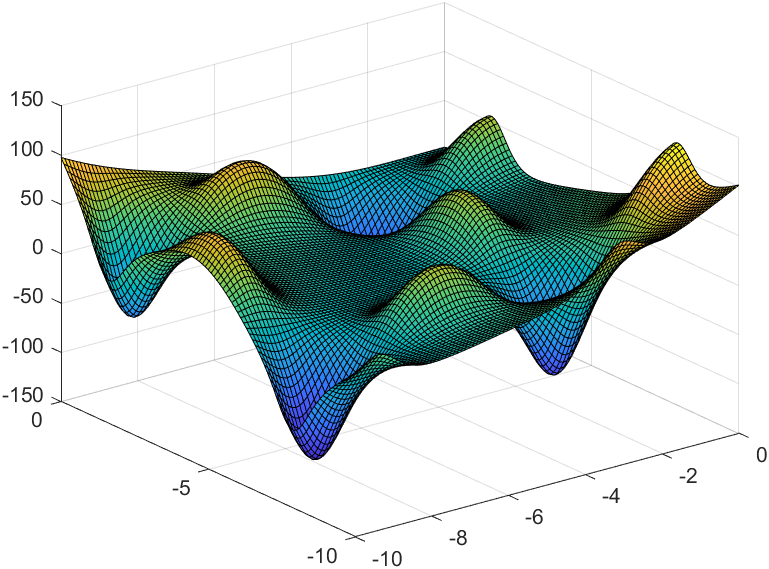
\includegraphics[width=0.4\textwidth]{assets/birdplot.png}
%     \caption{Grafik Tiga Dimensi Mirsha's Bird Function}
% \end{figure}

\begin{figure}[h!]
    \centering
    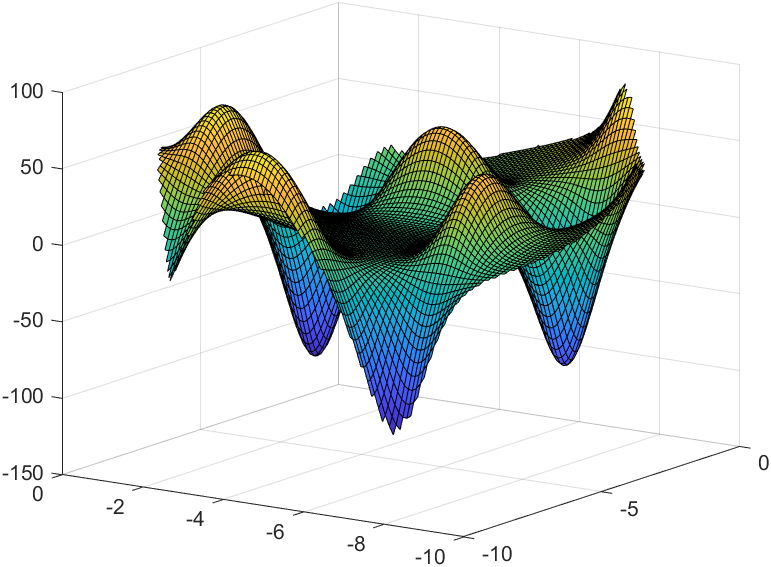
\includegraphics[width=0.4\textwidth]{assets/birdplotwithbound.png}
    \caption{Grafik Tiga Dimensi Mirsha's Bird Function dengan Kendala}
\end{figure}

\subsubsection*{D2.}
Mari kita teliti 2 kasus kemungkinan seperti yang dideskripsikan di pertanyaan soal.
\begin{itemize}
    \item Jika solusi minimum berada pada interior fungsi kendala, maka $g(x) \leq 0$ dan $\nabla \mathcal{L} = 0$. Fungsi kendala tidak 'berlaku' dan kita bisa menganggap $\lambda = 0$. 
    \item Jika solusi minimum berada pada \textit{boundary} dari fungsi kendala, maka $g(x) = 0$.
\end{itemize}
Dapat disimpulkan bahwa dalam kedua kasus ini, kita memiliki kondisi $\lambda g(x) = 0$. Maka masalah di soal ini adalah untuk mencari $\min_{x} f(\mathbf{x}) + \lambda g(\mathbf{x})$ dengan batasan $g(x) \leq 0$, $\lambda \geq 0$ dan $\lambda g(x) = 0$.

Maka dapat dibuat sistem persamaan nonlinear seperti di bawah ini:
$$
\psi (x, \lambda) = \begin{bmatrix}
    \nabla \mathcal{L}(x, \lambda) \\
    \lambda g(x)
\end{bmatrix}  = 0
$$

dan matriks Jacobian-nya:

$$
J (\vec{x}, \lambda) = \begin{bmatrix}
    H \mathcal{L}(\vec{x}, \lambda) & \nabla h(\vec{x}) \\
    \nabla (\lambda h(\vec{x}))^T & g(\vec{x})
\end{bmatrix}  = 0
$$

Untuk menyelesaikan masalah \textit{qudratic programming} di atas, digunakan iterasi Newton $\vec{x}_{k+1} = \vec{x}_k + s_x$ dan $\lambda_{k+1} = \lambda_k + s_{\lambda}$ dengan $s = (s_x, s_\lambda)$ solusi dari

$$
J(\vec{x}_k, \lambda_k)s = - \psi (\vec{x}_k, \lambda_k)
$$

Dengan tebakan awal $\vec{x_0} = [-3, -1.5]^T$, kita mendapatkan nilai $\vec{x} = [-3.130402085366371, -1.582423465940726]^T$ (nilai fungsi $-106.7645226519476$) setelah 10 iterasi. Berikut adalah tabel galat setiap iterasinya (dibandingkan dengan nilai minimum global $-106.764537$).

\begin{table}[H]
\centering
\begin{tabular}{|c|c|c|c|}
\hline
\textbf{Iterasi} & \textbf{Galat} & \textbf{Iterasi} & \textbf{Galat}  \\ \hline
$1$ & $-0.0209335200518694$ & $6$ & $-1.43480476282321e-05$ \\ \hline
$2$ & $-1.41035842631254e-05$ & $7$ & $-1.43217430093046e-05$ \\ \hline
$3$ & $-1.43217625492298e-05$ & $8$ & $-1.43480499872339e-05$ \\ \hline
$4$ & $-1.43480452976519e-05$ & $9$ & $-1.43217453540956e-05$ \\ \hline
$5$ & $-1.43217406787244e-05$ & $10$ & $-1.43480524030792e-05$\\ \hline
\end{tabular}
\end{table}

Bisa dilihat bahwa ada \textit{periodicity} disebabkan oleh sifat fungsi yang memiliki komponen periodik seperti $sin$ dan $cos$. Bila kita perhatikan pada matriks Hessiannya memiliki determinan positif dan kombinasi turunan keduanya $f_{xx}$ pada titik tersebut juga positif. Sehingga titik tersebut dapat disimpulkan merupakan lokal minimum.

Dari pengamatan plot juga, titik tersebut merupakan titik global minimum untuk \textit{constraint} yang diberikan. Secara umum, bila kita tidak memiliki \textit{plot tools}, maka kita dapat mengacak beberapa ratus tebakan awal, dan membandingkan nilai yang paling rendah. Setiap tebakan awal akan cenderung konvergen pada titik kritisnya. Secara matematika, tentunya salah satu titik-titik puncak tersebut akan berada pada titik kritisnya, kemudian akan dilakukan perbandingan terhadap semua titik kritis yang ditemukan. Secara probabilitas, kemungkinan mendapatkan titik-titik minimum ini akan cukup besar.

\nocite{*}
\bibliographystyle{apalike}
\bibliography{bibliography.bib}
\pagenumbering{gobble}
\end{document}